\subsection{Quantum Field Theory Axioms (A5--A6)}
%-----------------------------------------------------------------------------

\begin{tcolorbox}[colback=yellow!5, colframe=yellow!60!black, 
    title={\textbf{Conventions: Units, Masses, and Normalizations}}, fonttitle=\bfseries]

\textbf{Units and constants:}
\begin{itemize}[leftmargin=1.5em, topsep=2pt, itemsep=1pt]
    \item Natural units: $\hbar = c = 1$; energies in GeV, lengths in GeV$^{-1}$.
    \item Reference data: CODATA 2022, PDG 2024.
    \item Metric signature: $(+,-,-,-)$.
    \item Levi-Civita tensor: $\varepsilon^{0123} = +1$, $\tilde{F}^{\mu\nu} = \frac{1}{2}\varepsilon^{\mu\nu\rho\sigma}F_{\rho\sigma}$.
\end{itemize}

\textbf{Planck mass definitions:}
\begin{center}
\begin{tabular}{@{}lll@{}}
\toprule
\textbf{Symbol} & \textbf{Definition} & \textbf{Value}\\
\midrule
$M_{\mathrm{Pl}}$ (unreduced) & $G^{-1/2}$ & $1.221 \times 10^{19}$ GeV\\
$\Mpl$ (reduced) & $(8\pi G)^{-1/2}$ & $2.435 \times 10^{18}$ GeV\\
\bottomrule
\end{tabular}
\end{center}
\textbf{Convention:} Block formulas (Sec.~\ref{sec:e8}) use $M_{\mathrm{Pl}}$ (unreduced). 
Relation: $M_{\mathrm{Pl}} = \sqrt{8\pi}\,\Mpl$.

\textbf{Axion sector:}
\begin{itemize}[leftmargin=1.5em, topsep=2pt, itemsep=1pt]
    \item Axion field $a$: Dimensionless; define $\theta = 4\pi a$ with $2\pi$ periodicity. Physical field: $a_{\text{phys}} = f_a \cdot a$.
    \item Theta variable: $\theta = 4\pi a$, so $L_{\mathrm{int}} = (\theta/32\pi^2)\,F\tilde{F}$.
    \item Quantization: $(1/2\pi)\int F \in \mathbb{Z}$ and $(1/32\pi^2)\int F\wedge F \in \mathbb{Z}$.
    \item Chern--Simons term: $\mathcal{L} \supset \cthree\, a\, F\tilde{F}$ with $\cthree = 1/(8\pi)$.
    \item Coupling: $\gagg = -4\cthree$ is dimensionless; $g_{a\gamma\gamma}^{\text{(phys)}} = \gagg / f_a$ has dimension $[\text{energy}]^{-1}$.
    \item \textbf{Maxwell convention:} We define the field strength by the exterior derivative $F := dA$, i.e.\ $F_{AB}=2\partial_{[A}A_{B]}$, independent of the torsionful affine connection (we do not use $F_{AB}=2\hat{\nabla}_{[A}A_{B]}$). Therefore U(1) gauge invariance is exact in the electromagnetic sector.
\end{itemize}
\textbf{Shift invariance (one-line proof):} $\theta\mapsto \theta+2\pi$ gives $\Delta S=(2\pi)\,(1/32\pi^2)\int F\wedge F=2\pi Q$ with $Q\in\mathbb{Z}$.
\end{tcolorbox}

\begin{axiom}{Axion--Photon Anomaly Coupling}{APC}
The unique additional coupling in the low-energy effective theory is a 
pseudoscalar axion--photon interaction of the canonical form
\[
L_{\mathrm{int}}=-\frac{g_{a\gamma\gamma}}{4}\,a\,F_{AB}\tilde{F}^{AB},
\qquad g_{a\gamma\gamma}=-4\cthree,
\]
fixed by the abelian anomaly (Fujikawa method).

\tcblower
\textbf{Status:} Standard in anomaly physics; follows from chiral measure.
\textbf{Evidence:} \texttt{axion\_shift\_invariance\_audit}, \texttt{u1\_bundle\_normalization\_audit}, \texttt{standard\_convention\_mapping\_audit}.

\textbf{Consequence:} The kernel coupling is
\begin{equation}
    \cthree = \frac{1}{8\pi}
\end{equation}
with no remaining normalization freedom.
\end{axiom}

\begin{axiom}{Modulus Closure in Background-Field Gauge}{BFG}
We introduce a dimensionless coupling modulus $\sigma$ with electromagnetic kinetic function
\begin{equation}
    \mathcal{L} \supset -\frac{1}{4} f(\sigma)\,F_{\mu\nu}F^{\mu\nu}
    + \frac{1}{2}(\partial\sigma)^2,
    \qquad 
    \alpha(\sigma)=\frac{1}{4\pi f(\sigma)}.
\end{equation}
The physical vacuum extremizes the effective action with respect to $\sigma$:
\begin{equation}
    \frac{\delta\Gamma_{\mathrm{eff}}}{\delta\sigma}=0.
\end{equation}
In background-field gauge, the effective potential can be written as
$V_{\mathrm{eff}}(\sigma)=U(\alpha(\sigma)) + V_{\mathrm{geo}}(\sigma)$, where
$V_{\mathrm{geo}}'(\sigma_\star)=0$ by geometric closure.
If $\alpha(\sigma)$ is monotonic near the vacuum, this is equivalent to
\begin{equation}
    \frac{\partial U}{\partial \alpha}=0,
    \qquad U(\alpha)=U(\sigma(\alpha)).
\end{equation}

\tcblower
\textbf{Status:} Standard in modulus stabilization; background-field gauge provides a clean definition of $\Gamma_{\mathrm{eff}}$.

\textbf{Consequence:} $\alpha$ is fixed by a modulus extremum, not treated as a variational constant.
\end{axiom}

%-----------------------------------------------------------------------------
\subsection{Closure Axioms (A7--A8)}
%-----------------------------------------------------------------------------

\begin{axiom}{Standard Model Hypercharge Trace}{SMT}
We adopt the convention $Q=T_3+Y$ and count left-handed Weyl fermions plus the Higgs
scalar with their SU(2) and color multiplicities. Define the hypercharge trace
\begin{equation}
    b_Y = \frac{2}{3}\sum_{\text{Weyl}} d_3 d_2\,Y^2
    + \frac{1}{3}\sum_{\text{scalars}} d_3 d_2\,Y^2,
    \qquad
    \bone = \frac{3}{5}\,b_Y.
\end{equation}
Here $b_Y$ is the SM-normalized trace coefficient and $\bone$ is the corresponding
GUT-normalized coefficient used in the CFE.
For the SM field content (three generations + one Higgs doublet):
\begin{equation}
    Q:\tfrac{1}{3},\quad L:1,\quad u_c:\tfrac{8}{3},\quad d_c:\tfrac{2}{3},\quad e_c:2,\quad H:\tfrac{1}{6},
    \qquad b_Y=\frac{41}{6},\quad \bone=\frac{41}{10}.
\end{equation}
In TFPT this quantity appears as the \emph{spectral quadratic index} of the
hypercharge-coupled boundary operators in the regulated determinant
(Appendix~\ref{app:boundary}), not as an RG flow coefficient.

\tcblower
\textbf{Status:} Direct consequence of SM particle content; independent of RG scale.

\textbf{Important distinction:} $\bone$ is a \emph{hypercharge trace invariant}, 
not the one-loop beta function coefficient $b_1^{(\text{RG})}$. While numerically 
identical, their physical roles differ:
\begin{itemize}[leftmargin=1.5em, topsep=2pt, itemsep=1pt]
    \item $b_1^{(\text{RG})}$: Controls energy dependence $d\alpha_1/d\ln\mu$
    \item $\bone$ (TFPT): Discrete index counting charge content; scale-independent
\end{itemize}
\textbf{Bridge note:} $b_1$ enters the closure as a UV trace index; the observable mapping to $\alpha(0)$ is tracked explicitly in the bridge ledger.

\textbf{Consequence:} No exotic particles or modified charge structure required.
\end{axiom}

\begin{tcolorbox}[colback=yellow!3, colframe=yellow!60!black,
    title={\textbf{EW mapping (kernel $\alpha$ vs. observable $\alpha_{\mathrm{EM}}$)}}, fonttitle=\bfseries\small]
\textbf{Charge basis:} the discrete trace coefficient $b_1$ is computed in GUT-normalized hypercharge basis (A7).
\textbf{Bridge bookkeeping:} electroweak relations track the mapping between $\alpha(0)$, $\overline{\alpha}^{(5)}(M_Z)$, and $(g_Y,g_2)$ conventions.
\textbf{GUT normalization:} $\alpha_Y = \tfrac{3}{5}\alpha_1$.
\textbf{EW identity:} $\alpha_{\mathrm{EM}}^{-1} = \alpha_1^{-1} + \alpha_2^{-1}$, i.e.\ $1/e^2=1/g_Y^2+1/g_2^2$.
\textbf{Status:} these identities are enforced by \texttt{ew\_mixing\_mapping\_audit} and \texttt{thomson\_limit\_matching\_audit}.
\end{tcolorbox}

\begin{figure}[H]
\centering
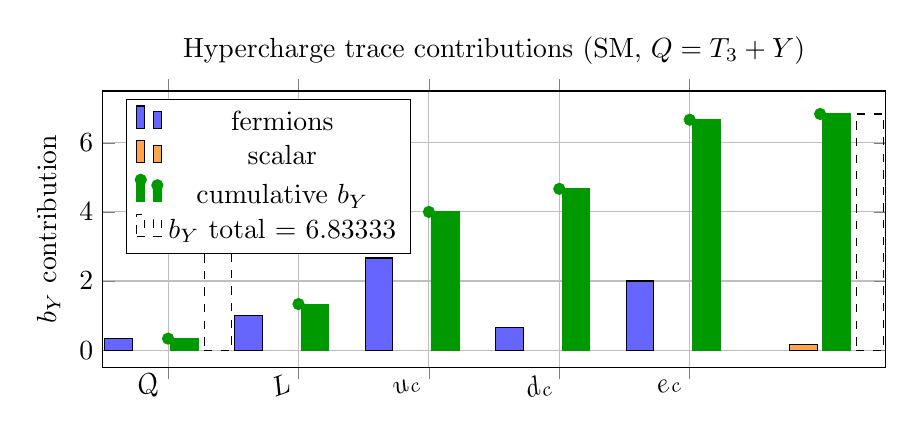
\begin{tikzpicture}
\begin{axis}[
    ybar,
    width=0.95\linewidth,
    height=0.42\linewidth,
    ylabel={$b_Y$ contribution},
    title={Hypercharge trace contributions (SM, $Q=T_3+Y$)},
    symbolic x coords={Q,L,uc,dc,ec,H},
    xtick=data,
    xticklabel style={rotate=20,anchor=east},
    xticklabels={$Q$,$L$,$u_c$,$d_c$,$e_c$,$H$},
    grid=major,
    legend pos=north west
]
\addplot[fill=blue!60] coordinates {
    (Q,0.3333333333333333)
    (L,1.0)
    (uc,2.6666666666666665)
    (dc,0.6666666666666666)
    (ec,2.0)
};
\addlegendentry{fermions}
\addplot[fill=orange!70] coordinates {(H,0.16666666666666666)};
\addlegendentry{scalar}
\addplot+[mark=*, color=green!60!black] coordinates {
    (Q,0.3333333333333333)
    (L,1.3333333333333333)
    (uc,4.0)
    (dc,4.666666666666667)
    (ec,6.666666666666667)
    (H,6.833333333333333)
};
\addlegendentry{cumulative $b_Y$}
\addplot[black, dashed] coordinates {(Q,6.833333333333333) (H,6.833333333333333)};
\addlegendentry{$b_Y$ total = 6.83333}
\end{axis}
\end{tikzpicture}
\caption{Hypercharge trace contributions by SM field. The explicit Weyl+Higgs sum closes the definition of $b_1=41/10$ under $Q=T_3+Y$.}
\label{fig:b1-trace}
\end{figure}

\begin{tcolorbox}[colback=yellow!3, colframe=yellow!50!black, 
    title={\textbf{Scale Consistency: Why $\bone$ (UV) Determines $\alpha$ (IR)}}, fonttitle=\bfseries\small]
\textbf{Potential objection:} The abelian trace $\bone = 41/10$ is computed from the full SM spectrum 
(quarks, leptons, gauge bosons) at high energies. How can it determine $\alpha$ in the Thomson 
limit ($Q^2 \to 0$)?

\textbf{Resolution:} The CFE is a stationarity (closure) condition for the effective action; it is \emph{not} an RG differential equation.

\begin{enumerate}[leftmargin=1.5em, topsep=2pt, itemsep=1pt]
    \item \textbf{Spectral origin:} In the APS framework with flat $U(1)_Y$ holonomies on the boundary cycles,
        the regulated determinant produces a universal trace coefficient proportional to $\sum_f Y_f^2$.
        Thresholds affect non-universal finite terms, not this discrete spectral index.
    \item \textbf{Field-content fixed coefficient:} $\bone$ is the GUT-normalized hypercharge trace 
        $\frac{5}{3}\sum_f Y_f^2$ of the full SM spectrum. Once the field content and charge assignments are fixed, 
        $\bone$ is a discrete input and does not ``run'' as a function of $\mu$.
    \item \textbf{UV log coefficient, not IR running:} In the one-loop effective action, $\bone$ multiplies the UV logarithmic term 
        coming from the abelian charge trace. TFPT uses this UV coefficient inside the stationarity condition; it does not attempt to compute 
        the infrared running $\alpha(\mu)$.
    \item \textbf{Threshold independence (anomaly matching):} Below mass thresholds, particles decouple from IR loops, but the UV charge-trace 
        coefficient is fixed by the UV-complete spectrum. The sum $41/10$ is the asymptotic value and remains the relevant discrete input.
    \item \textbf{CFE vs.\ RG:} Standard RG asks ``how does $\alpha(\mu)$ evolve?'' The CFE asks ``what value of $\alpha$ makes the effective action stationary 
        given $(\cthree,\phiz,\bone)$?'' It is a closure condition, not a flow equation.
\end{enumerate}

\textbf{Reviewer-safe statement:} We use $\bone$ as the discrete spectral trace coefficient of the
hypercharge-coupled boundary operators in the UV logarithmic term of the regulated determinant.
TFPT explicitly does \emph{not} claim to compute the IR running $\alpha(\mu)$ or threshold matching.

\textbf{Prediction:} If additional charged particles exist beyond the SM (e.g., SUSY partners), 
$\bone$ would change and the CFE would predict a \emph{different} $\alpha$. This is testable.
\end{tcolorbox}

\begin{axiom}{GR Renormalization Condition}{GRN}
In the torsion-free limit ($K \to 0$), the theory must exactly reproduce 
Einstein--Hilbert gravity.

\tcblower
\textbf{Status:} Physical consistency requirement.

\textbf{Consequence:} Fixes the gravitational coupling structure:
$\kappa^2 = 8\pi G$, with the dimensionless ratio $\xi = \cthree/\phiz$ constrained by topology.
The dimensional scale $M_{\mathrm{Pl}}$ remains an external input.
\end{axiom}

%=============================================================================
\section{Derivation of Fundamental Constants}
%=============================================================================

%-----------------------------------------------------------------------------
\subsection{\texorpdfstring{The Geometric Scale $\phiz$}{The Geometric Scale phi0}}
%-----------------------------------------------------------------------------

\begin{theorem}{Existence and Uniqueness of $\phiz$}{phi0}
From Axioms A3 and A4, the geometric scale is uniquely determined:
\begin{equation}
    \phiz = \phitree + \deltatop = \frac{1}{6\pi} + \frac{3}{256\pi^4} = \num[round-mode=places,round-precision=17]{\TFPTvarphiZeroNum}
\end{equation}
\end{theorem}

\begin{proof}
From A3 ($\eta$-gluing): the M\"obius double cover contributes two physical boundary
cycles ($2\pi+2\pi$) plus a discrete seam gluing term ($2\pi$), giving
$R_{\text{total}}=6\pi$. The closure normalization $\chi = \varphi R = 1$
yields $\phitree = 1/(6\pi)$.
Here $\varphi$ is the dimensionless geometry modulus of the M\"obius reduction; the
normalization fixes its scale and can be taken as an explicit geometric-closure axiom.
Physical predictions depend only on dimensionless ratios and the discrete increments.

From A4: the unique gauge-invariant correction at leading order is 
$\deltatop = 48\cthree^4 = 3/(256\pi^4)$.
\end{proof}

\begin{tcolorbox}[colback=gray!5, colframe=gray!60, breakable,
    title={\textbf{Dictionary: $\beta_{\text{rad}}$ and Canonical Consequences}}, fonttitle=\bfseries\small]
\textbf{Definition (notation):}
\[
\beta_{\text{rad}} := \frac{\phiz}{4\pi}.
\]
\textit{Note:} dimensionless; equals the birefringence angle in radians for the minimal topological excursion $\Delta a_{\text{top}}=\phiz$.

\textbf{Immediate algebraic consequences:}
\begin{equation}
    \phiz = 4\pi\beta_{\text{rad}}, 
    \qquad 
    \beta_{\text{deg}} := \frac{180}{\pi}\,\beta_{\text{rad}}.
\end{equation}
\begin{equation}
    \gagg = -4\cthree = -\frac{1}{2\pi},
    \qquad
    \deltatop = 48\cthree^4 = \frac{3}{256\pi^4}.
\end{equation}

\textbf{Remark:} Many later ``$\beta_{\text{rad}}$-centric'' relations are compact rewrites of earlier definitions. 
We catalogue their logical status (definition vs.\ consequence vs.\ lemma vs.\ prediction) in Appendix~\ref{app:identities}.
\end{tcolorbox}

% Suite-extracted invariant table (high precision)
\TFPTCoreInvariantTable

%-----------------------------------------------------------------------------
